\begin{apendicesenv}

\partapendices

\chapter{Mapeamento e Justificativa do Processo }\label{apendice:mapeamento}

Neste apêndice está presente o framework desenvolvido pela equipe do trabalho, para criação das atividades de engenharia de requisitos,
com base no Scaled Agile Framework, Rational Unified Process , Melhoria de Processo de Software Brasileiro e Atividades Fundamentais da Engenharia de Requisitos.


\begin{figure}[H]
    \centering
	\includegraphics[keepaspectratio=true,scale=0.85]{figuras/mapeamento/Mapeamento_1.eps}
    \caption{Mapeamento de Atividades Parte 1.}
    \label{fig:processo}
\end{figure}

\begin{figure}[H]
    \centering
	\includegraphics[keepaspectratio=true,scale=0.85]{figuras/mapeamento/Mapeamento_2.eps}
    \caption{Mapeamento de Atividades Parte 2.}
    \label{fig:processo}
\end{figure}

\begin{figure}[H]
    \centering
	\includegraphics[keepaspectratio=true,scale=0.85]{figuras/mapeamento/Mapeamento_3.eps}
    \caption{Mapeamento de Atividades Parte 3.}
    \label{fig:processo}
\end{figure}

\chapter{Evoluções do Processo}\label{apendice:evolution}

Para se chegar na versão final do processo criado, foram realizadas 7 iterações, desde uma modelagem de baixa fidelidade, até a
modelagem de acordo com os padrões BPMN. Em todas as iterações se obteve a consultoria do Orientador do trabalho. As evoluções foram registradas e serão representadas nas figuras abaixo:

\begin{figure}[H]
    \centering
	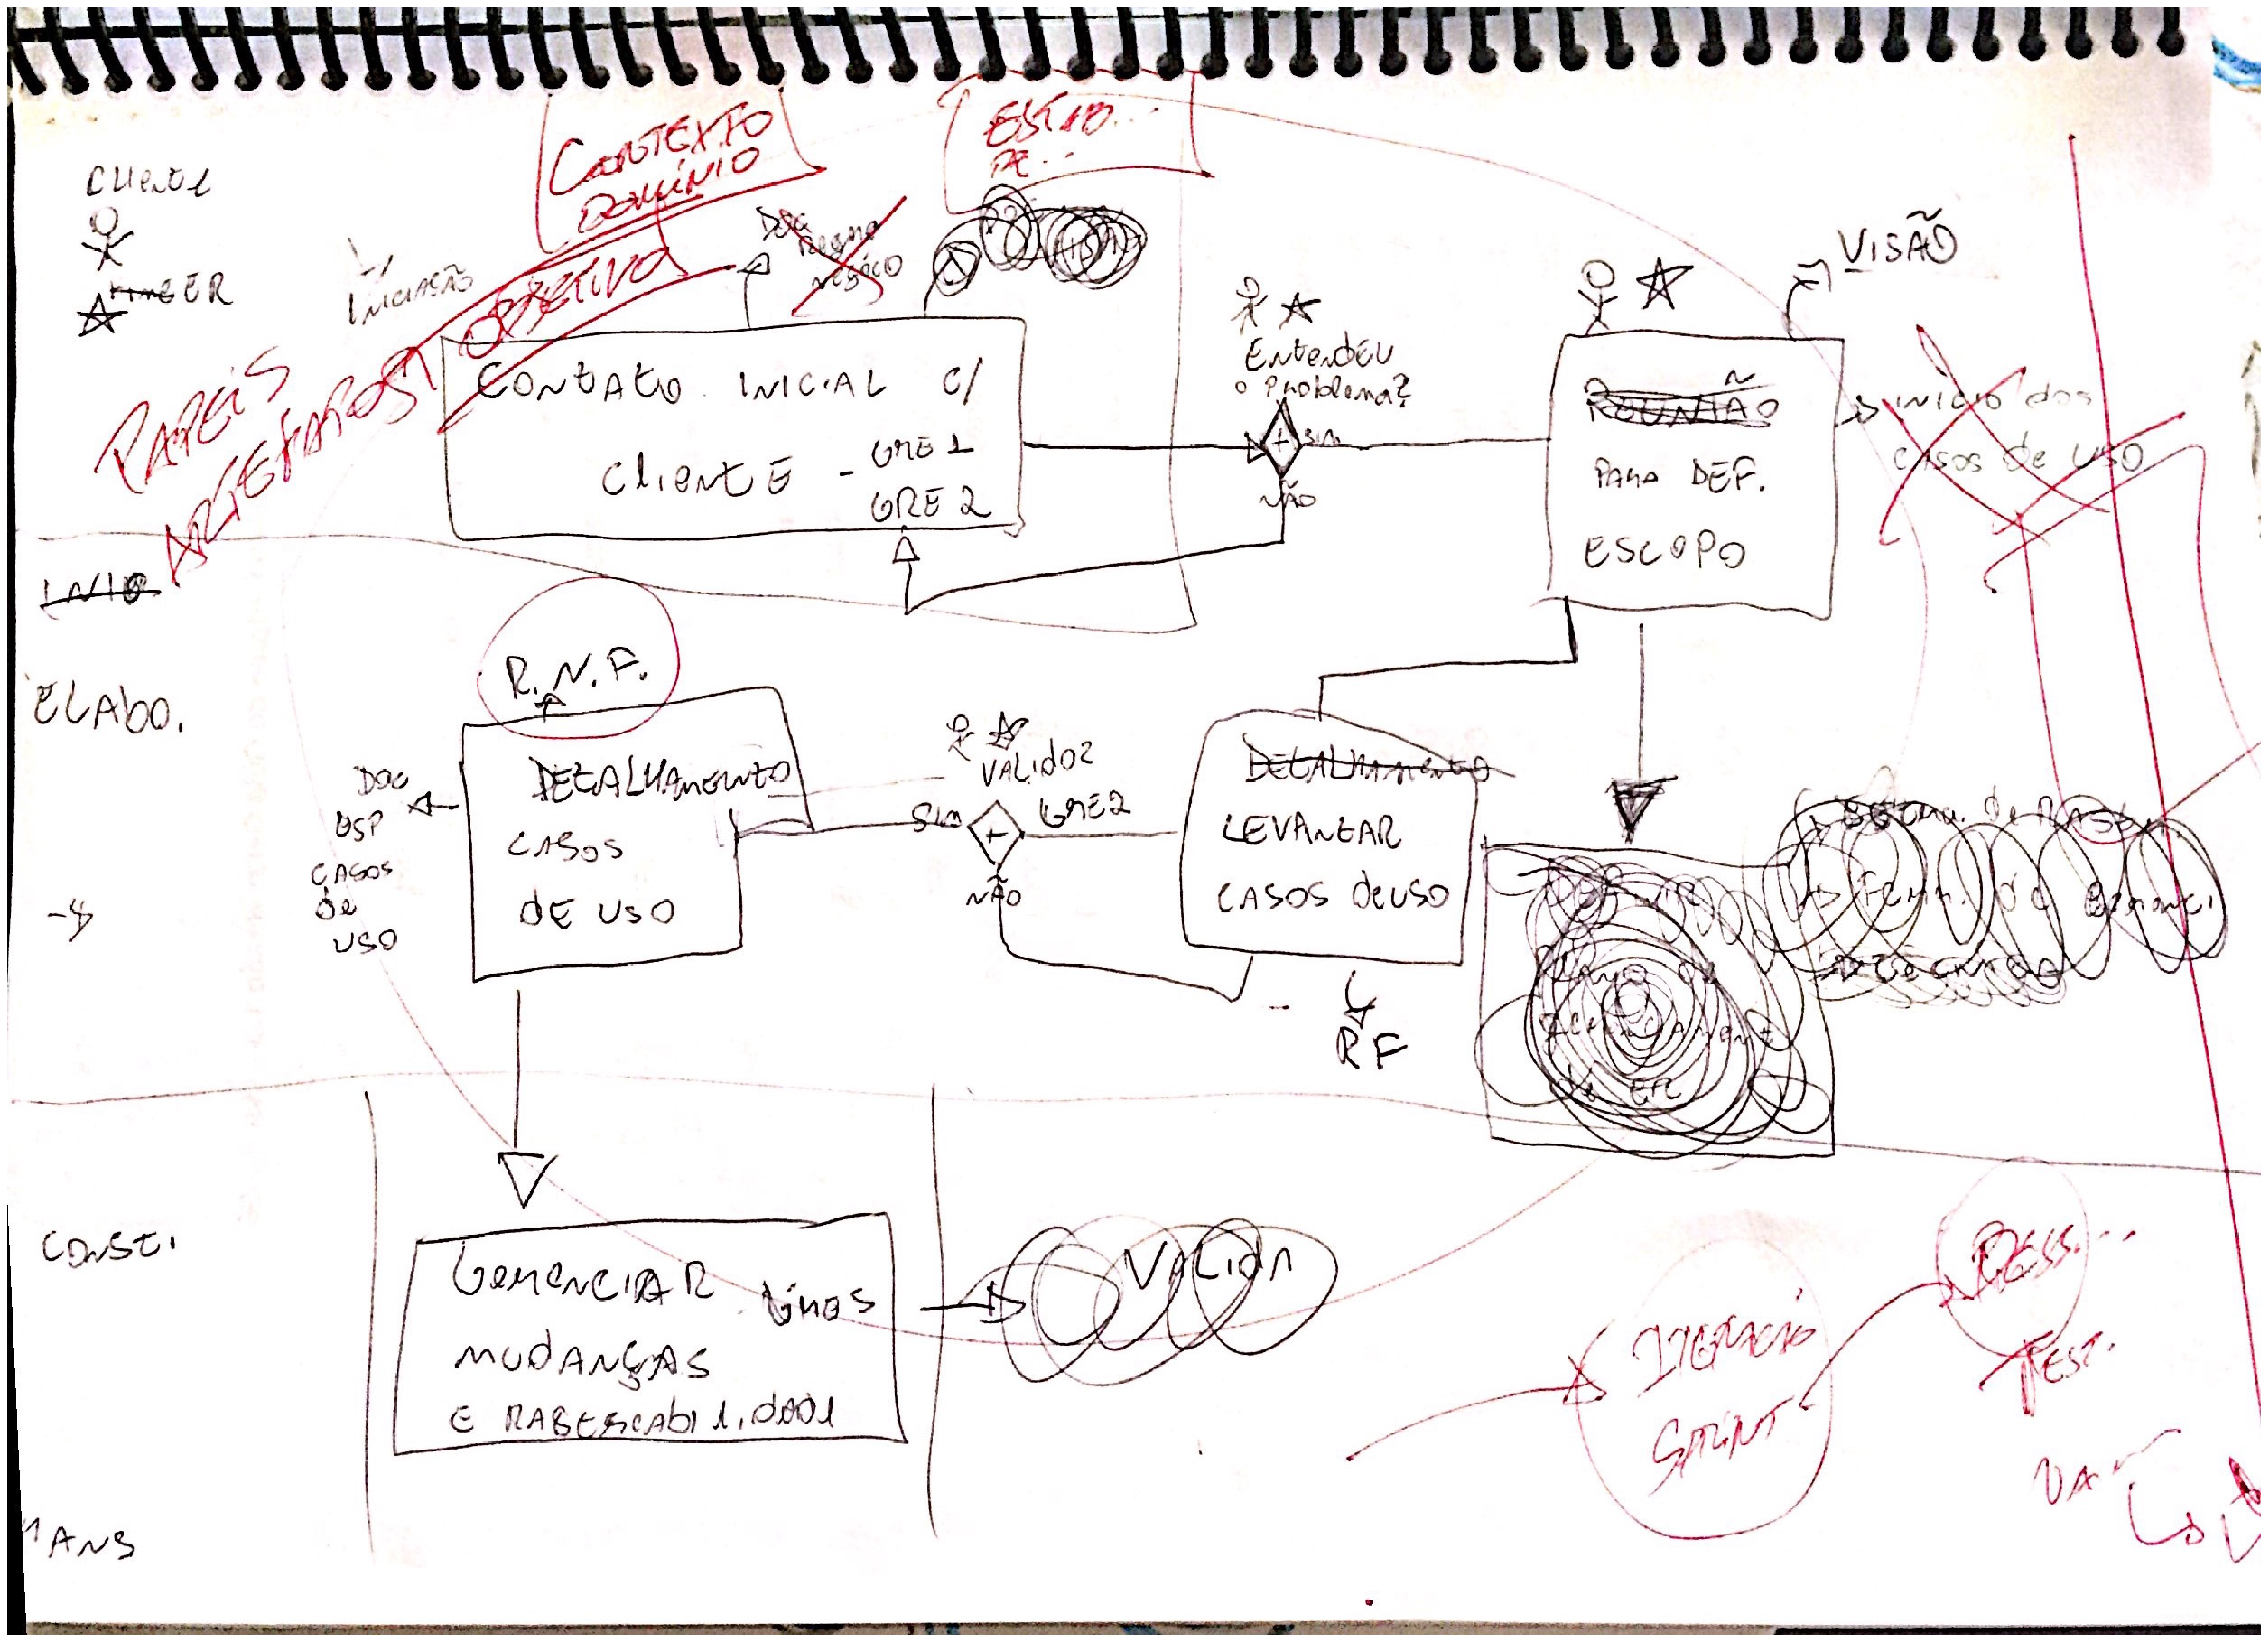
\includegraphics[keepaspectratio=true,scale=0.17]{figuras/evolucao_processo/Processo_v0.eps}
    \caption{Versão esboço inicial do processo criado.}
    \label{fig:processo}
\end{figure}

\begin{figure}[H]
    \centering
	\includegraphics[keepaspectratio=true,scale=0.5]{figuras/evolucao_processo/Processo_v1.eps}
    \caption{Versão 1 do processo criado.}
    \label{fig:processo}
\end{figure}

\begin{figure}[H]
    \centering
	\includegraphics[keepaspectratio=true,scale=0.5]{figuras/evolucao_processo/Processo_v2.eps}
    \caption{Versão 2 do processo criado.}
    \label{fig:processo}
\end{figure}


\begin{figure}[H]
    \centering
	\includegraphics[keepaspectratio=true,scale=0.5]{figuras/evolucao_processo/Processo_v3.eps}
    \caption{Versão 3 do processo criado.}
    \label{fig:processo}
\end{figure}

\begin{figure}[H]
    \centering
	\includegraphics[keepaspectratio=true,scale=0.5]{figuras/evolucao_processo/Processo_v4.eps}
    \caption{Versão 4 do processo criado.}
    \label{fig:processo}
\end{figure}

\begin{figure}[H]
    \centering
	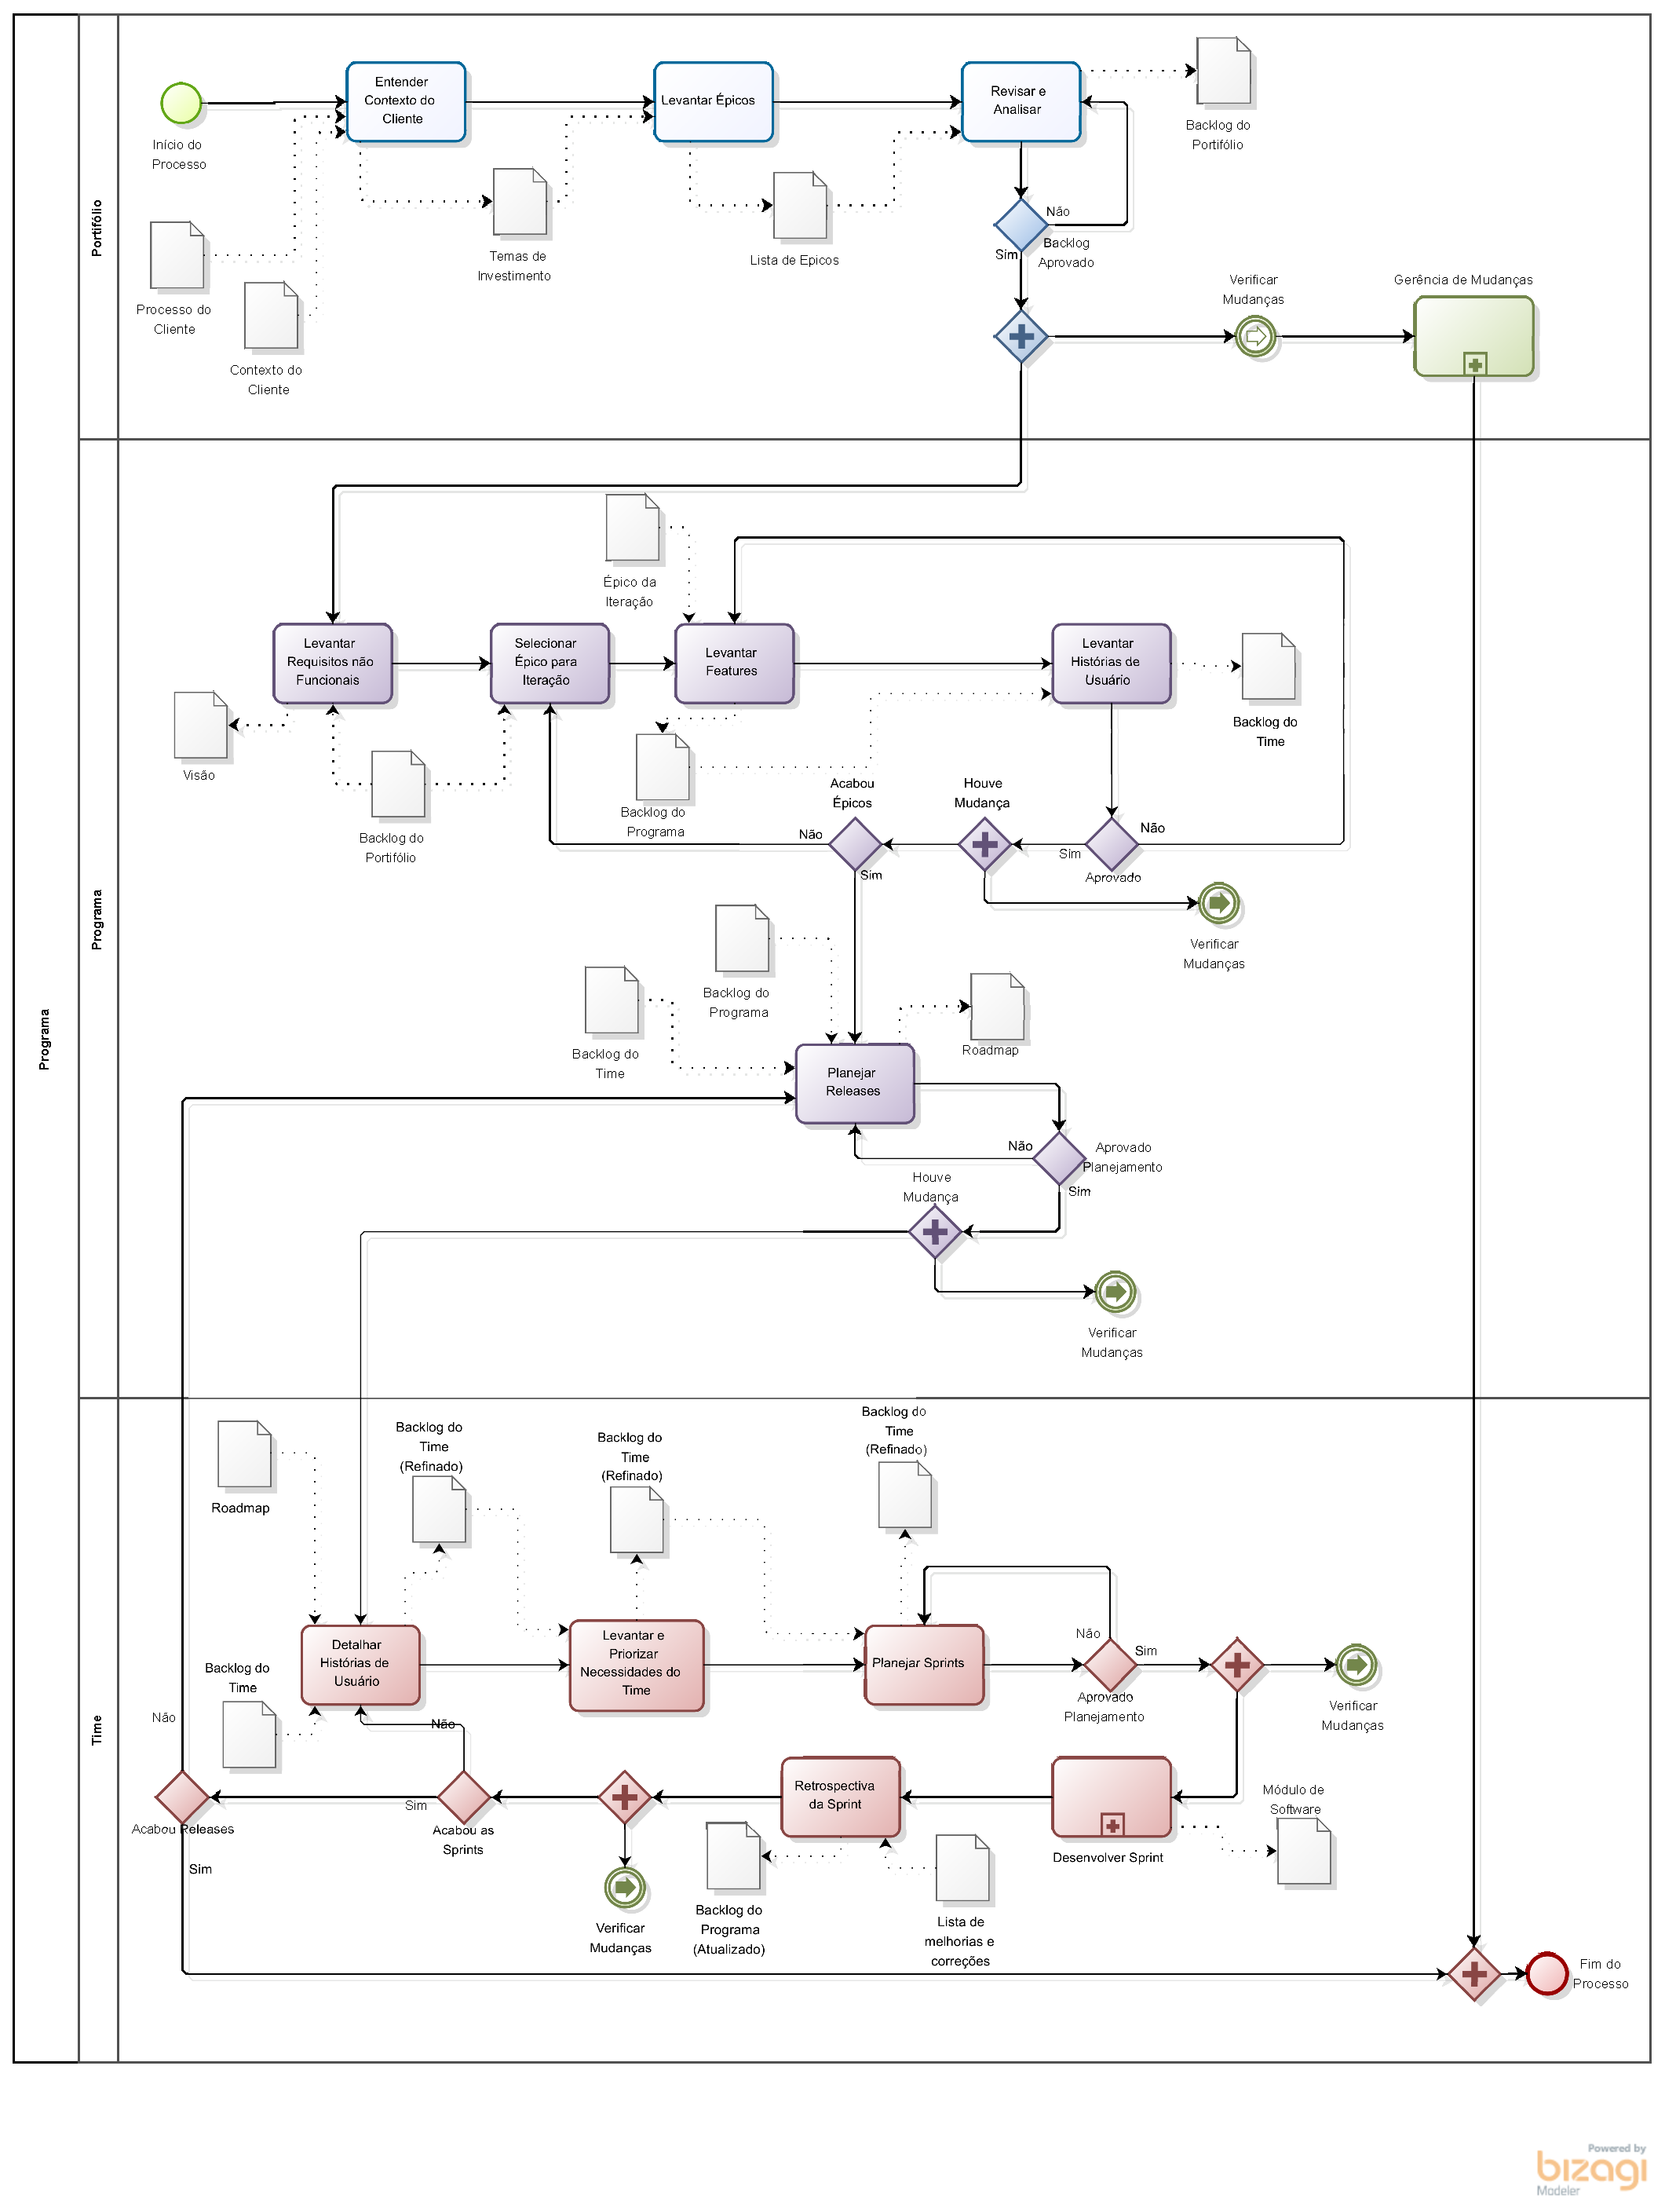
\includegraphics[keepaspectratio=true,scale=0.52]{figuras/evolucao_processo/Processo_v5_1.eps}
    \caption{Versão 5 do processo criado.}
    \label{fig:processo}
\end{figure}

\begin{figure}[H]
    \centering
	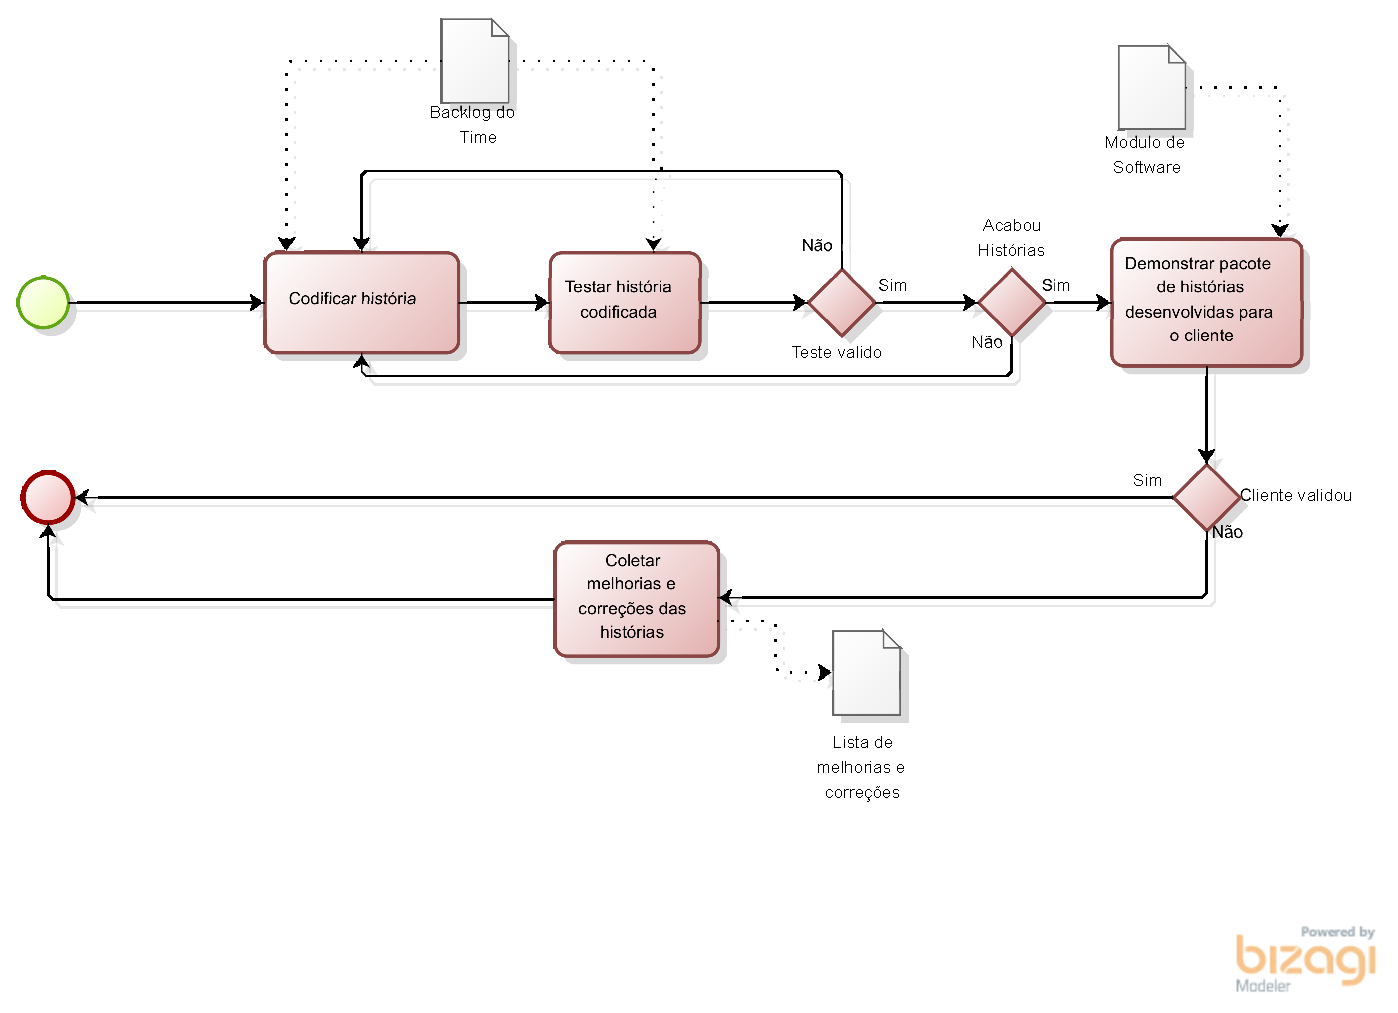
\includegraphics[keepaspectratio=true,scale=0.53]{figuras/evolucao_processo/Processo_v5_2.eps}
    \caption{Versão 5 do processo criado. Sub Processo Desenvolvimento. }
    \label{fig:processo}
\end{figure}

\begin{figure}[H]
    \centering
	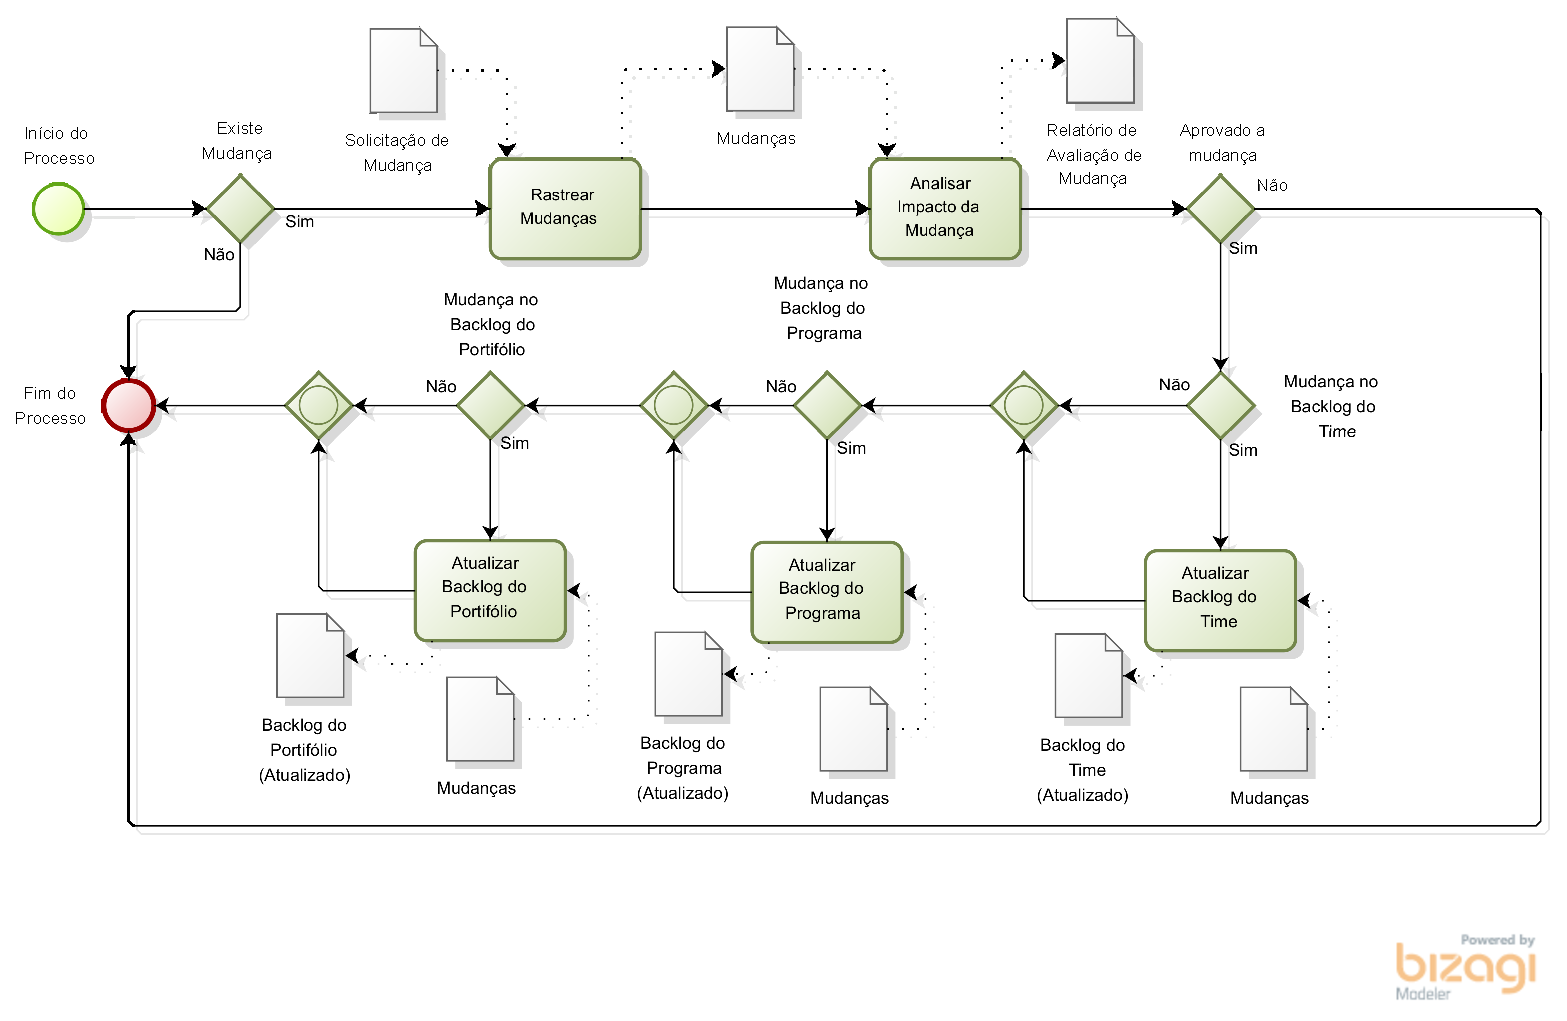
\includegraphics[keepaspectratio=true,scale=0.53]{figuras/evolucao_processo/Processo_v5_3.eps}
    \caption{Versão 5 do processo criado. Sub Processo Gerência de Mudanças }
    \label{fig:processo}
\end{figure}

\chapter{Templates de Artefatos}\label{apendice:templates}

Texto do apendice c

\chapter{Processo atual de manutenção de software do MC}\label{apendice:current_process_mc}

  Abaixo uma modelagem na notação BPMN do proceso atual da manutenção de software do Ministério das Comunicações.

\begin{figure}[H]
    \centering
	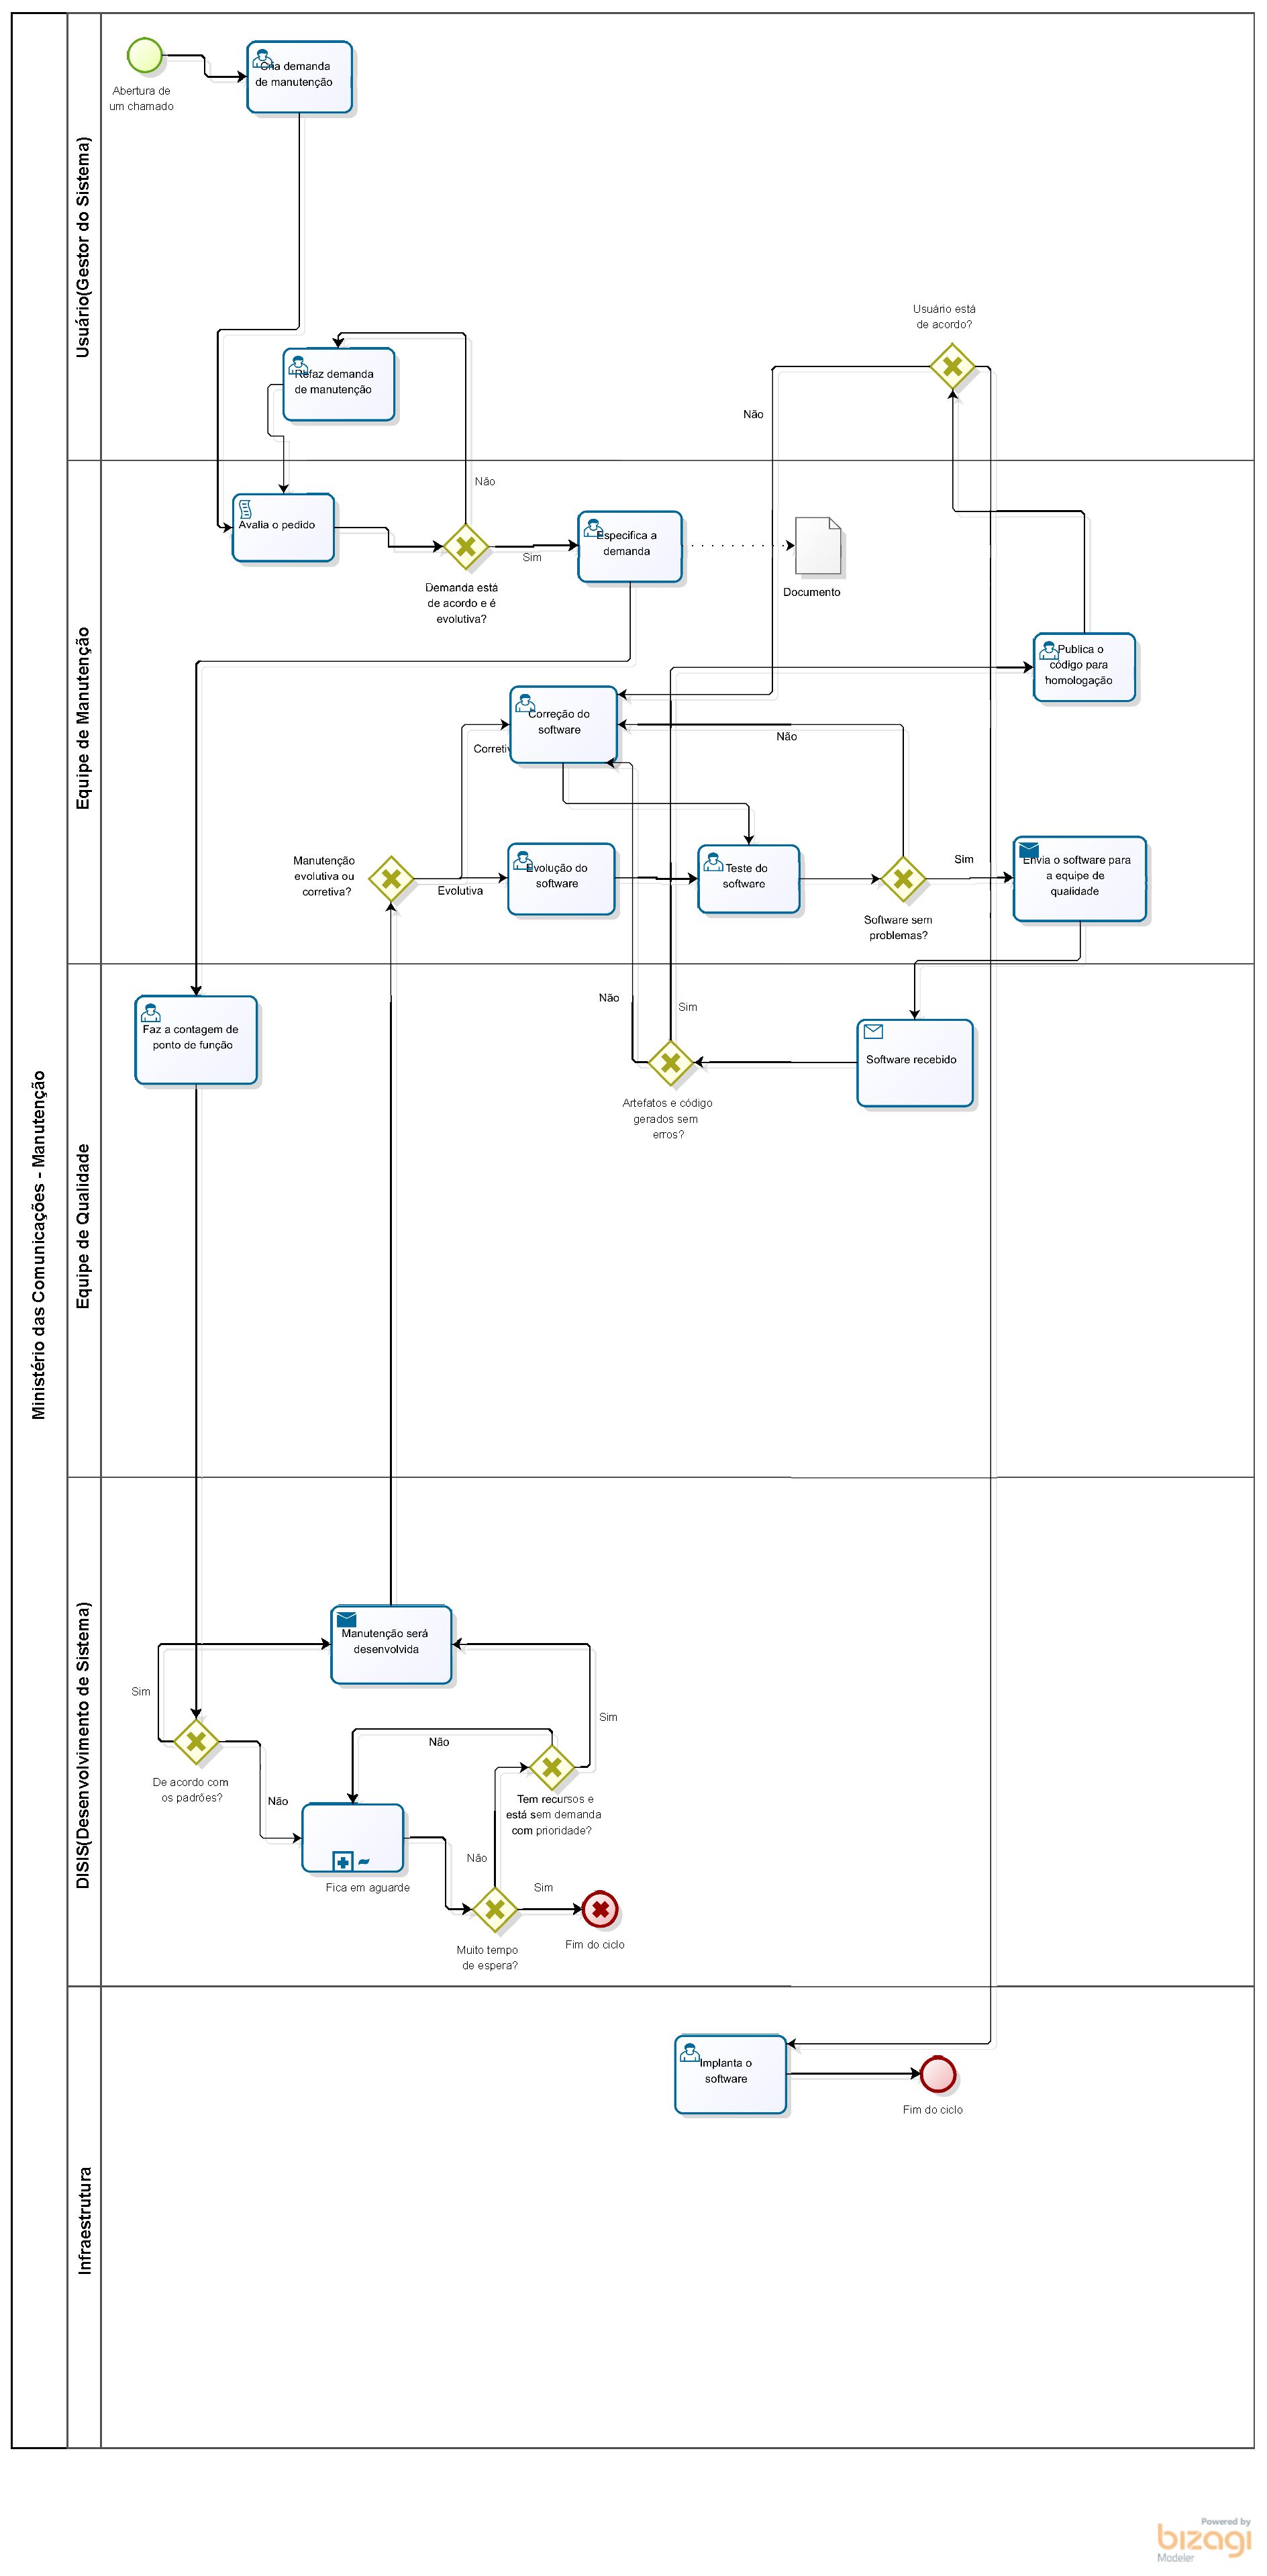
\includegraphics[keepaspectratio=true,scale=0.35]{figuras/MC_Processo_Atual.eps}
    \caption{Processo atual de manutenção de software do MC}
    \label{fig:process_atual_mc}
\end{figure}

\end{apendicesenv}
